% ============================================================
%  CHAPITRE 3 : CONCEPTION ARCHITECTURALE DE LA PLATEFORME

\chapter{Conception architecturale de la plateforme}

\minitoc

\newpage

\section{Introduction}

Les concepts présentés dans le chapitre précédent ont permis d'établir les fondements théoriques nécessaires à la conception de la plateforme. À partir de ces bases, il est désormais possible de définir l'architecture de la solution proposée.

Ce chapitre présente l'architecture globale de la plateforme, notamment son organisation microservices, son modèle multi-tenant, son modèle de données ainsi que l'intégration des agents d'intelligence artificielle. Il expose également les principaux choix technologiques retenus et les raisons ayant motivé leur adoption.

\section{Architecture de la plateforme}

Cette section présente l'architecture globale de la plateforme. Elle décrit la structuration du système en différentes couches, en mettant en évidence la séparation entre l'interface utilisateur, la logique métier, les composants d'intelligence artificielle, ainsi que la gestion des données et de la mémoire.

\subsection{Vue d'ensemble de l'architecture}

La plateforme repose sur une architecture en couches afin de structurer le système de manière
claire et évolutive. Cette vue d'ensemble permet de présenter les principales responsabilités de
la solution ainsi que les échanges entre ses composants.

\subsubsection{Organisation générale des couches}

L'architecture est structurée autour de six couches principales, comme l'illustre la
figure~\ref{fig:platform_layered_architecture}. Elles sont présentées de haut en bas selon le
parcours d'une requête dans le système :

\begin{enumerate}
    \item \textbf{Couche de présentation :} elle correspond à l'interface web utilisée par les
    différents profils de la plateforme. Elle permet d'afficher les données, de déclencher les
    actions utilisateur et de communiquer avec le backend à travers des appels API.

    \item \textbf{Couche API Gateway :} elle constitue le point d'entrée unique entre
    l'interface web et les services internes. Elle reçoit les requêtes du frontend, les redirige
    vers le service approprié et centralise l'accès aux fonctionnalités backend.

    \item \textbf{Couche des microservices :} elle regroupe les services responsables des
    principaux domaines fonctionnels de la plateforme, tels que l'identité, l'administration,
    la gestion des cours, le suivi de progression et la gamification. Elle applique les règles
    métier et prépare les données nécessaires aux traitements du système.

    \item \textbf{Couche IA :} elle regroupe les agents spécialisés responsables des traitements
    intelligents de la plateforme, comme la création assistée de cours, le coaching, la
    mémorisation, la recommandation et la génération de défis personnalisés.

    \item \textbf{Couche Hindsight :} elle constitue la couche de mémoire persistante utilisée
    par les agents IA. Elle permet de conserver et de récupérer les informations utiles à la
    personnalisation des traitements.

    \item \textbf{Couche de données :} elle regroupe les systèmes de stockage utilisés par la
    plateforme, notamment PostgreSQL et les composants nécessaires à la persistance des
    données métier, des historiques et des résultats produits par le système.
\end{enumerate}

\begin{figure}[H]
    \centering
    \IfFileExists{figures/platform_layered_architecture.png}{%
        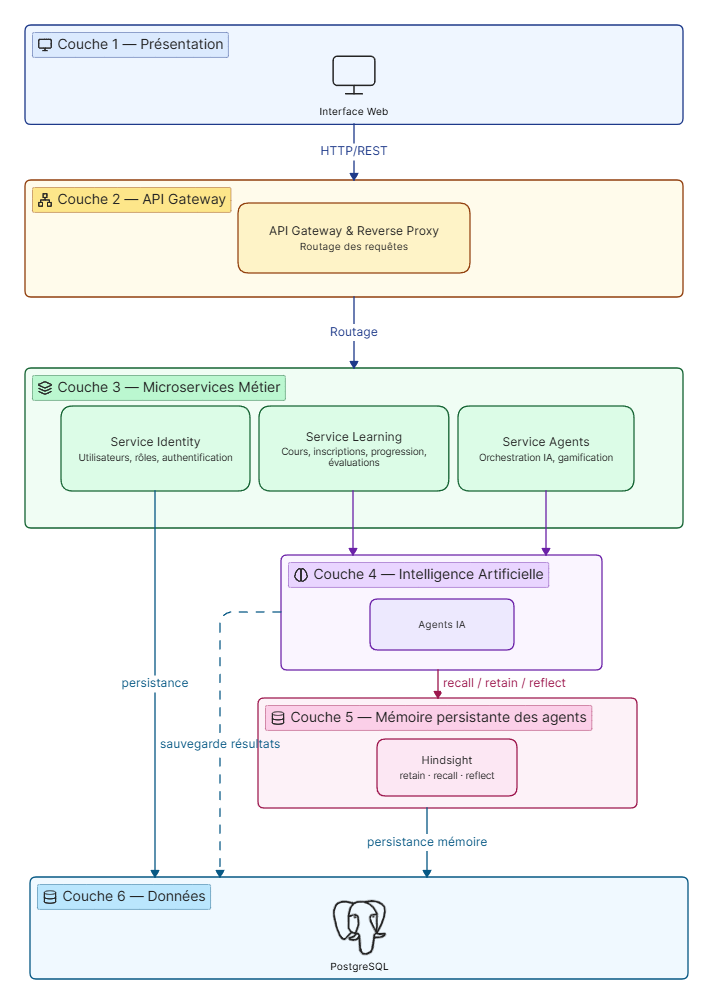
\includegraphics[width=0.95\textwidth,height=0.72\textheight,keepaspectratio]{figures/platform_layered_architecture.png}
    }{%
        \fbox{\parbox{0.85\textwidth}{\centering Schéma d'architecture en couches à insérer ici.}}
    }
    \caption{Vue d'ensemble de l'architecture en couches de la plateforme}
    \label{fig:platform_layered_architecture}
\end{figure}

\subsubsection{Articulation entre les couches}

Ces six couches s'articulent de manière progressive. L'utilisateur interagit avec la couche de présentation, qui envoie ses requêtes vers l'\textit{API Gateway}. Celle-ci transmet les appels aux microservices concernés. Lorsque le traitement nécessite une personnalisation ou une génération intelligente, les microservices sollicitent la couche IA. Les agents peuvent alors récupérer ou enrichir le contexte à travers Hindsight, puis retourner le résultat vers les services métier. Les données nécessaires au suivi applicatif sont ensuite stockées dans la couche de données, tandis que les traces utiles à la personnalisation sont conservées dans la mémoire persistante.

\subsubsection{Séparation entre logique métier et logique IA}

Cette organisation met en évidence une séparation importante entre la logique métier et la logique IA. Les microservices restent responsables des règles fonctionnelles de la plateforme, alors que les agents IA sont responsables des traitements intelligents liés au contenu, à l'accompagnement et à la personnalisation. Cette séparation rend l'architecture plus lisible, facilite l'évolution des agents et limite l'impact d'une modification IA sur le fonctionnement métier de la plateforme.

Les sous-sections suivantes détaillent ensuite les deux parties principales de cette architecture : l'organisation microservices du backend, puis l'architecture des agents IA et leurs workflows.

\subsection{Architecture microservices du backend}

L'architecture backend de la plateforme repose sur une approche microservices. Ce choix permet d'éviter un backend monolithique dans lequel l'authentification, la gestion pédagogique, le suivi des apprenants et les traitements IA seraient regroupés dans une seule application. La plateforme couvre plusieurs domaines fonctionnels distincts ; il est donc plus adapté de séparer ces responsabilités afin de faciliter la maintenance, l'évolution et le déploiement progressif des fonctionnalités.

Dans ce projet, le backend est structuré autour de quatre services principaux :
\textit{Identity}, \textit{Learning}, \textit{Agents} et \textit{API Gateway}. Ce découpage permet
d'introduire les principaux composants backend qui seront détaillés dans les sous-sections
suivantes.

\subsubsection{API Gateway}

L'accès aux microservices est centralisé à travers une couche \textit{API Gateway}. Traefik, utilisé comme reverse proxy \cite{traefik_official}, est chargé de recevoir les requêtes entrantes et de les rediriger vers le microservice approprié selon les règles de routage définies. Cette couche reçoit les requêtes provenant du frontend, applique les règles de routage et transmet chaque appel vers le service approprié. Elle permet donc au frontend de communiquer avec un point d'entrée unique au lieu de connaître directement les adresses internes des services. Elle facilite aussi l'organisation des routes API, l'isolation des services dans le réseau Docker et l'évolution de l'architecture lorsqu'un nouveau service est ajouté.

\subsubsection{Microservices réels et modules fonctionnels internes}

Dans l'implémentation de la plateforme, le backend n'est pas découpé en microservices pour chaque fonctionnalité. Il repose sur trois microservices principaux : \textit{identity}, \textit{learning} et \textit{agents} (Figure~\ref{fig:backend_microservices_components}). Les différentes fonctionnalités sont organisées sous forme de modules internes rattachés à ces services.

\begin{itemize}
    \item \textbf{Microservice identity :} Ce microservice couvre tout le domaine lié à l'identité et à l'accès à la plateforme. Il inclut l'authentification, la gestion des utilisateurs, des rôles, des tenants ainsi que les journaux d'audit. Il représente le point central de contrôle des accès et des permissions.

    \item \textbf{Microservice learning :} Ce microservice regroupe le domaine pédagogique de la plateforme, incluant les cours, les leçons, la progression, les quiz, la gamification ainsi que les recommandations et les défis. Ces fonctionnalités sont gérées comme des modules internes et peuvent interagir avec la couche IA lorsque nécessaire.

    \item \textbf{Microservice agents :} Ce microservice est dédié aux agents IA et adopte une granularité plus fine. Les agents ne sont pas des services indépendants, mais des composants logiques orchestrés au sein du même service. Chaque agent dispose de son propre prompt, de ses skills et de ses outils.
\end{itemize}

Le microservice agents joue un rôle d'orchestrateur central : il reçoit les requêtes, sélectionne l'agent approprié, initialise son contexte et retourne le résultat généré.

\begin{figure}[H]
    \centering
    \IfFileExists{figures/backend_microservices_components.png}{%
        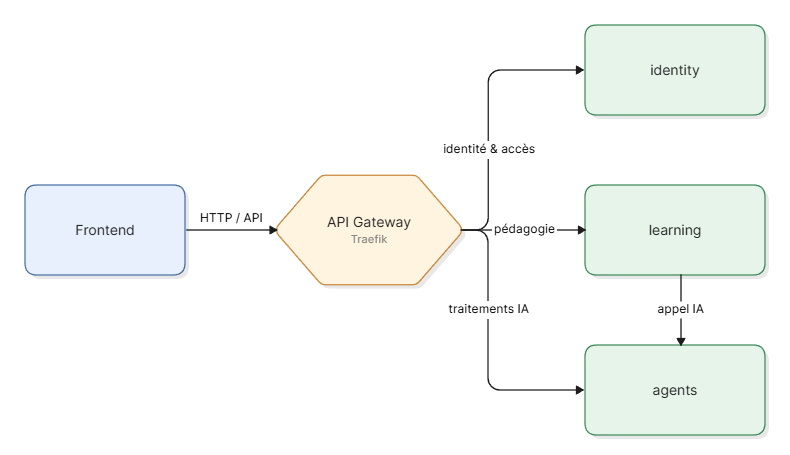
\includegraphics[width=0.85\textwidth,keepaspectratio]{figures/backend_microservices_components.png}
    }{%
        \fbox{\parbox{0.85\textwidth}{\centering Diagramme de composants UML des microservices backend à insérer ici.}}
    }
    \caption{Organisation des microservices du backend}
    \label{fig:backend_microservices_components}
\end{figure}

\subsection{Architecture multi-tenant}

Une architecture multi-tenant permet à plusieurs organisations de partager une même plateforme tout en assurant une séparation logique de leurs données et de leurs utilisateurs \cite{medimagh_multitenant}.

Dans ce projet, cette approche répond au contexte du Groupe 3S, où plusieurs sociétés utilisent la même plateforme de formation tout en conservant leurs propres utilisateurs, cours et données de suivi.

L'isolation des données est assurée par l'utilisation d'un identifiant de tenant (\textit{tenant\_id}) associé aux entités métier. Ce mécanisme permet de restreindre l'accès aux données de chaque organisation et de garantir une séparation stricte entre les différents tenants.

La figure~\ref{fig:multi_tenant_architecture} présente l'organisation générale de l'architecture multi-tenant mise en place dans la plateforme. Elle illustre le partage de l'infrastructure applicative entre plusieurs entreprises tout en assurant l'isolation logique des données de chaque tenant.

\begin{figure}[H]
    \centering
    \IfFileExists{figures/Architecture_multi-tenant_plateforme.png}{%
        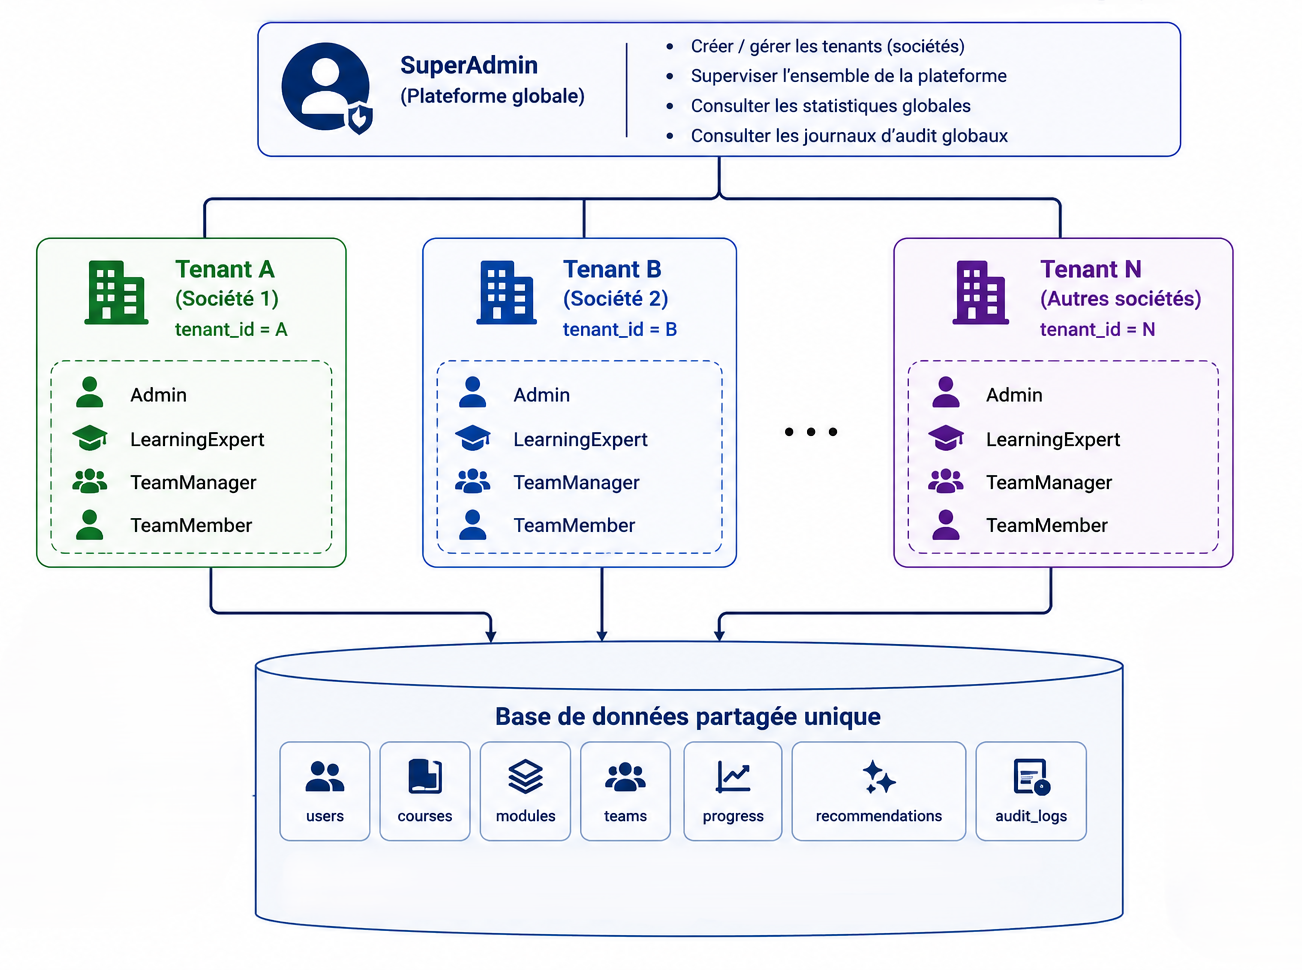
\includegraphics[width=0.8\textwidth]{figures/Architecture_multi-tenant_plateforme.png}
    }{%
        \fbox{\parbox{0.85\textwidth}{\centering Architecture multi-tenant de la plateforme à insérer ici.}}
    }
    \caption{Architecture multi-tenant de la plateforme}
    \label{fig:multi_tenant_architecture}
\end{figure}

La gestion des accès est également organisée au niveau du tenant. Chaque organisation dispose de ses propres utilisateurs et de ses propres rôles. Les utilisateurs peuvent accéder uniquement aux ressources appartenant à leur tenant, tandis qu'un rôle Super Admin dispose d'une visibilité globale sur l'ensemble des tenants du système.

La figure~\ref{fig:multi_tenant_use_case} illustre les différents acteurs et leurs interactions avec les fonctionnalités de la plateforme à l'intérieur d'un tenant.

\begin{figure}[H]
    \centering
    \IfFileExists{figures/diagrammeUC.png}{%
        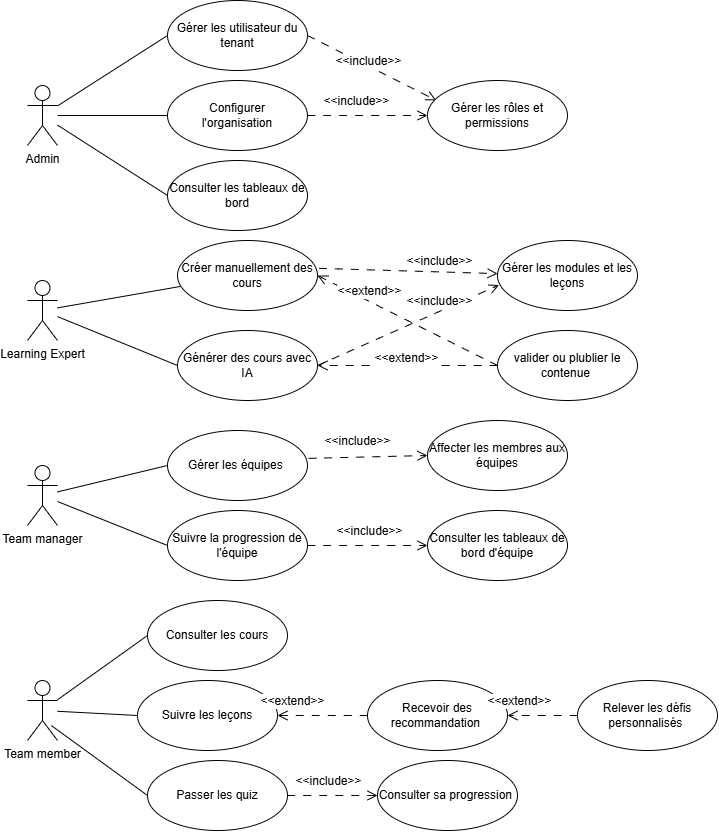
\includegraphics[width=0.72\textwidth]{figures/diagrammeUC.png}
    }{%
        \fbox{\parbox{0.85\textwidth}{\centering Diagramme de cas d'utilisation UML des acteurs au sein d'un tenant à insérer ici.}}
    }
    \caption{Diagramme de cas d'utilisation UML des acteurs au sein d'un tenant}
    \label{fig:multi_tenant_use_case}
\end{figure}

\subsection{Modèle de données}

Le modèle de données repose sur une base relationnelle PostgreSQL, utilisée pour le stockage des principales informations métier de la plateforme, notamment les utilisateurs, les organisations, les cours, les inscriptions, la progression, les évaluations ainsi que les fonctionnalités intelligentes telles que les recommandations et les défis personnalisés. Ce choix garantit la cohérence des données et leur intégrité dans un contexte multi-tenant.

Les données de la plateforme peuvent être regroupées en plusieurs catégories fonctionnelles, incluant les informations d'identité et d'administration des organisations, les contenus pédagogiques (cours, modules, leçons et évaluations), les données de suivi de l'apprentissage (inscriptions, progression et résultats), ainsi que les données liées aux fonctionnalités intelligentes.

Par ailleurs, la plateforme adopte une approche de stockage hybride. Les données structurées et les métadonnées sont stockées dans PostgreSQL, tandis que les ressources pédagogiques volumineuses (vidéos, images, documents et supports de cours) sont externalisées dans MinIO. La base de données conserve uniquement les références vers ces ressources, ce qui permet d'optimiser les performances et de simplifier la gestion des contenus.

Ainsi, ce modèle de données combine la robustesse d'une base relationnelle avec la flexibilité d'un stockage objet, en adéquation avec les besoins fonctionnels et techniques de la plateforme.

\subsection{Architecture des agents IA}

La couche IA de la plateforme est organisée autour de plusieurs agents spécialisés, chacun associé à une responsabilité pédagogique précise. L'objectif n'est pas de construire un seul agent généraliste chargé de toutes les tâches, mais de répartir les traitements intelligents entre des agents plus ciblés : agent de création de cours, agent de coaching pédagogique, agent de mémoire apprenant, agent de recommandation et agent de défis personnalisés. Cette séparation permet de mieux contrôler le comportement de chaque agent et d'adapter ses consignes au contexte fonctionnel dans lequel il intervient.

\subsubsection{Agent de création de cours}

Cet agent assure la génération assistée des cours à travers une orchestration autour d'OpenMAIC. À partir d'une consigne fournie par l'expert pédagogique, éventuellement accompagnée d'un document PDF, il prépare la demande, suit l'exécution du processus et récupère le brouillon produit. OpenMAIC prend en charge la génération principale du contenu pédagogique, notamment les scènes de cours, les diapositives, les scripts du professeur, les quiz et, lorsque c'est pertinent, les activités interactives. Le résultat n'est pas un fichier statique, mais un brouillon structuré et éditable, ensuite sauvegardé dans la plateforme afin d'être révisé, validé puis transformé en cours officiel. Après la validation finale, le cours peut être enrichi par la génération audio TTS et transmis au Course Memory Agent pour son intégration dans la mémoire persistante. Le déroulement détaillé de cet agent est illustré par la figure \ref{fig:course_maker_agent_workflow}.

\begin{figure}[H]
    \centering
    \IfFileExists{figures/course_maker_agent_workflow.png}{%
        \makebox[\textwidth][c]{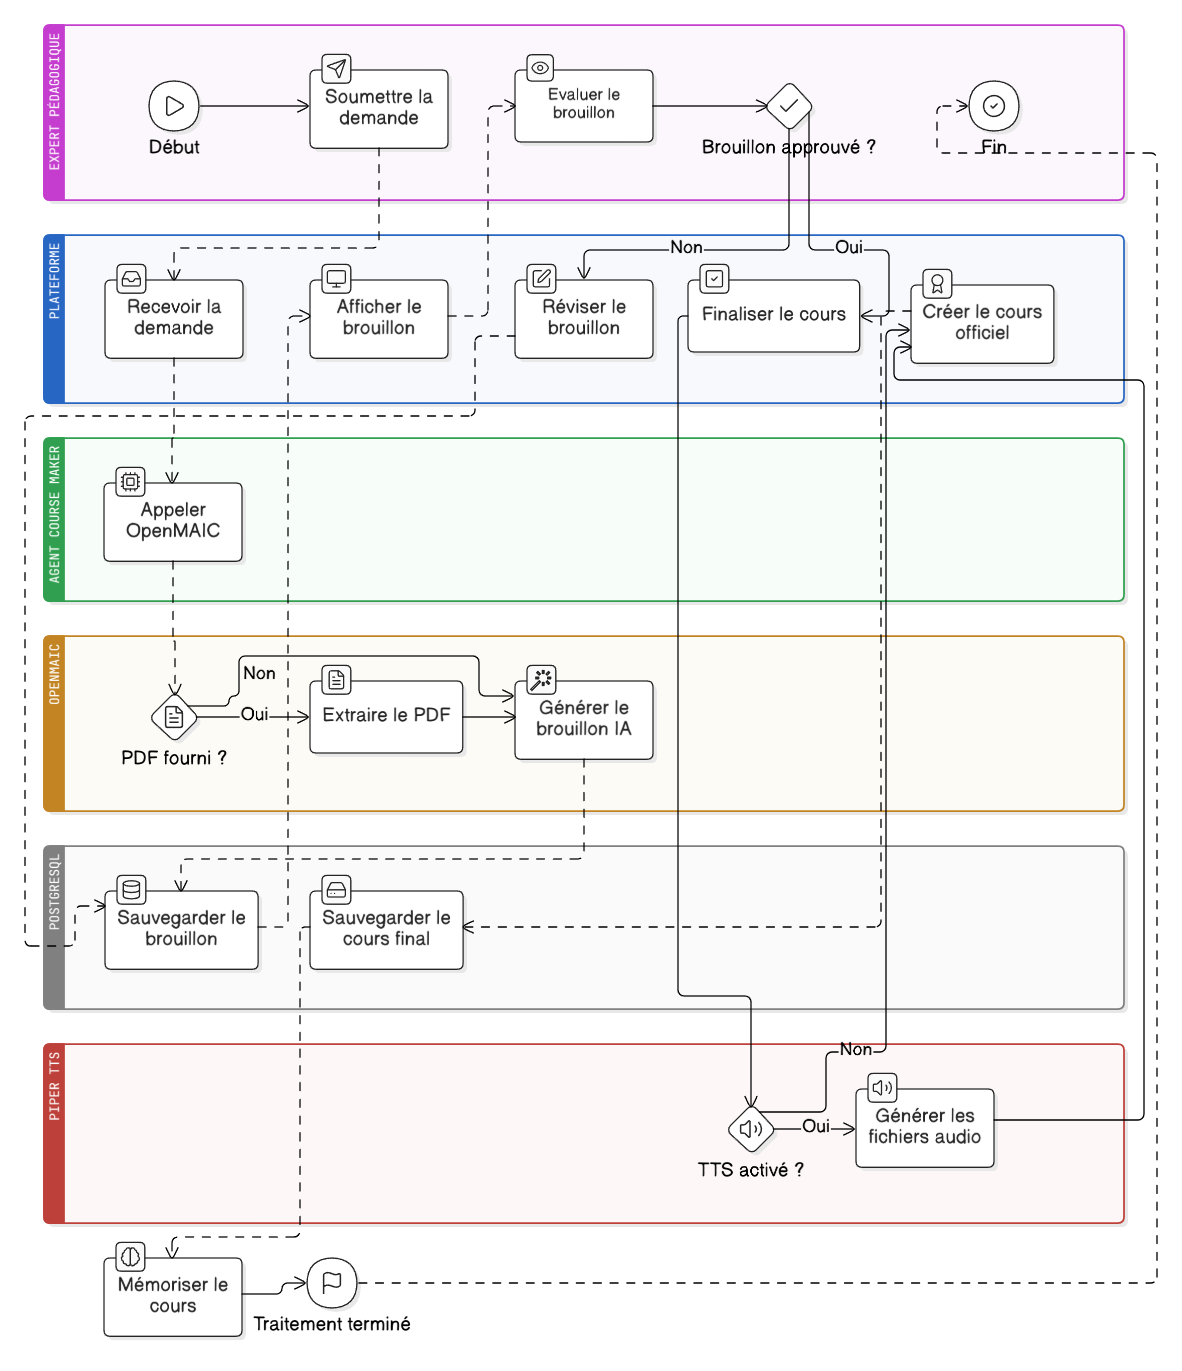
\includegraphics[width=1.05\textwidth,height=0.72\textheight,keepaspectratio]{figures/course_maker_agent_workflow.png}}
    }{%
        \fbox{\parbox{0.85\textwidth}{\centering Diagramme d'activité UML de l'agent de création de cours à insérer ici.}}
    }
    \caption{Diagramme d'activité UML de l'agent de création de cours}
    \label{fig:course_maker_agent_workflow}
\end{figure}

\subsubsection{Agent de coaching pédagogique}

Cet agent accompagne l'apprenant pendant son parcours en répondant à ses questions à partir du contexte du cours et de sa mémoire personnelle. Lorsqu'une question est posée, la plateforme transmet la demande à l'agent \textit{AI Coaching Agent}. Celui-ci récupère d'abord les informations pertinentes du cours à travers l'opération \textit{recall} de Hindsight, tout en déclenchant la mémorisation de la question de l'apprenant via l'agent de mémoire apprenant. Les éléments rappelés sont ensuite utilisés pour construire une requête enrichie, puis Hindsight exécute une opération \textit{reflect} sur la mémoire propre à l'apprenant et au cours. La réponse produite est ainsi contextualisée, liée au contenu pédagogique et adaptée à l'historique de l'utilisateur. Le déroulement de cet agent est illustré par la figure \ref{fig:ai_coaching_agent_workflow}.

\begin{figure}[H]
    \centering
    \IfFileExists{figures/ai_coaching_agent_workflow.png}{%
        \makebox[\textwidth][c]{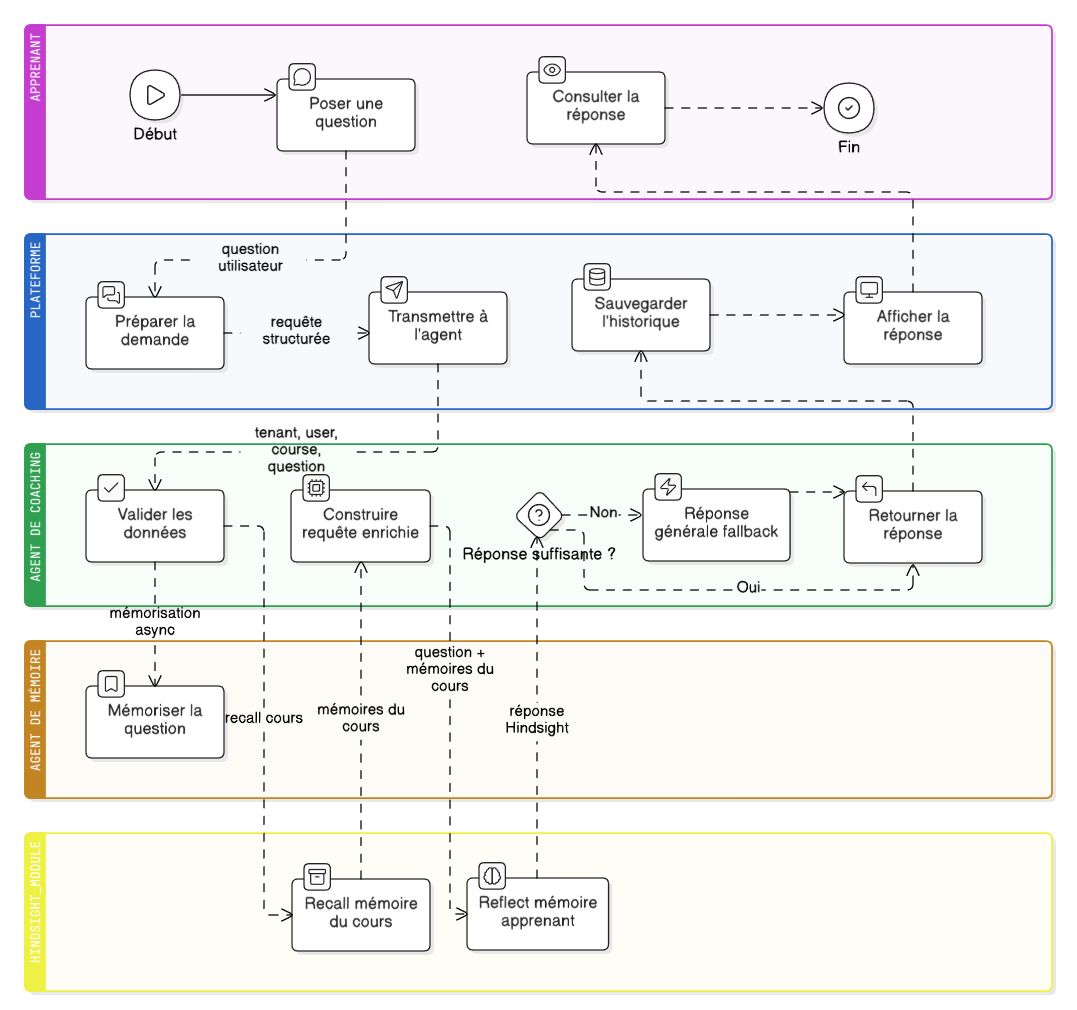
\includegraphics[width=1.02\textwidth,height=0.70\textheight,keepaspectratio]{figures/ai_coaching_agent_workflow.png}}
    }{%
        \fbox{\parbox{0.85\textwidth}{\centering Diagramme d'activité UML de l'agent de coaching pédagogique à insérer ici.}}
    }
    \caption{Diagramme d'activité UML de l'agent de coaching pédagogique}
    \label{fig:ai_coaching_agent_workflow}
\end{figure}

\subsubsection{Agent de mémoire apprenant}

Cet agent alimente la mémoire persistante du suivi pédagogique. Il est déclenché par plusieurs événements du parcours apprenant, comme l'envoi d'un message au \textit{AI Coaching Agent}, la complétion d'une leçon, le passage d'un quiz, la progression dans une vidéo, la détection d'une difficulté, la réponse à un défi personnalisé ou la complétion d'un cours. Après validation des données reçues, il prépare le contenu à mémoriser. Pour les messages de coaching, il vérifie les mémoires similaires avec \textit{recall} afin d'éviter les doublons, puis conserve les nouvelles informations avec \textit{retain}. Pour les autres événements d'apprentissage, il enregistre une trace structurée dans la banque mémoire de l'apprenant et du cours. Ces informations peuvent ensuite être rappelées par les autres agents pour personnaliser leurs réponses. Le fonctionnement de cet agent est illustré par la figure~\ref{fig:learner_memory_agent_workflow}.

\begin{figure}[H]
    \centering
    \IfFileExists{figures/learner_memory_agent_workflow.png}{%
        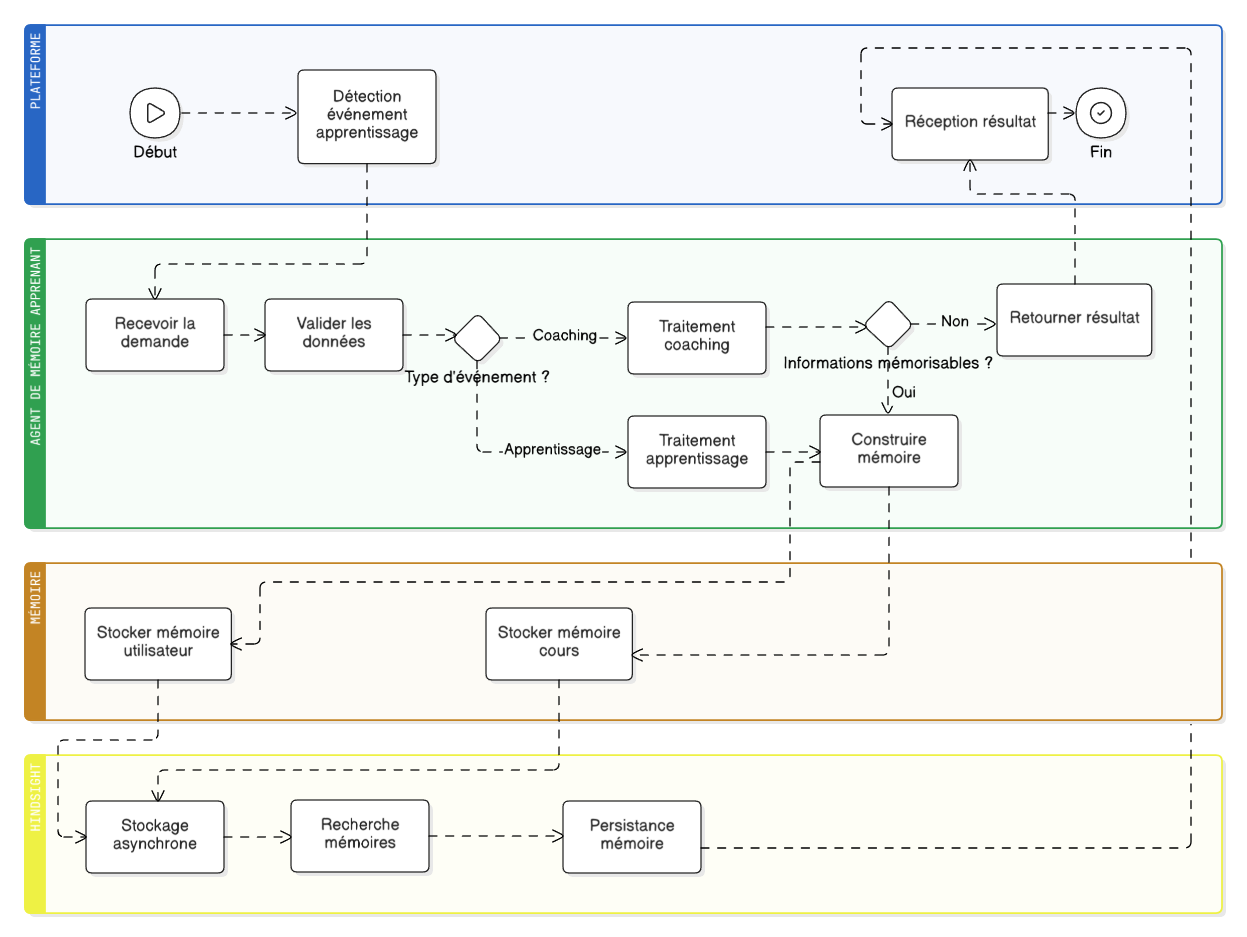
\includegraphics[width=\textwidth]{figures/learner_memory_agent_workflow.png}
    }{%
        \fbox{\parbox{0.85\textwidth}{\centering Diagramme d'activité UML de l'agent de mémoire apprenant à insérer ici.}}
    }
    \caption{Diagramme d'activité UML de l'agent de mémoire apprenant}
    \label{fig:learner_memory_agent_workflow}
\end{figure}

\subsubsection{Agent de recommandation}

Cet agent a pour objectif de personnaliser le parcours d'apprentissage en proposant à chaque apprenant les actions les plus adaptées à son état actuel. Il s'appuie d'abord sur les mémoires liées aux cours suivis par l'apprenant afin de construire un \textit{skill gap radar}, c'est-à-dire une synthèse des domaines de compétences maîtrisés, partiellement maîtrisés ou encore faibles. Les compétences faibles sont ensuite comparées avec le catalogue des cours publiés. Cette comparaison ne repose pas uniquement sur une décision manuelle : Hindsight et le LLM interviennent pour transformer les signaux d'apprentissage en domaines de compétences, tandis que l'agent applique ensuite une logique de correspondance par mots-clés entre ces compétences et les informations des cours, comme le titre, la description, la catégorie et le niveau. Pour chaque cours candidat, un score de pertinence est calculé selon le nombre de mots-clés communs, l'état de la compétence détectée et la situation de l'apprenant dans le cours. Par exemple, une compétence non maîtrisée reçoit une priorité plus forte, tandis qu'un cours déjà terminé est moins favorisé. Si le score obtenu dépasse le seuil défini, l'agent génère une recommandation de cours, de leçon ou de révision selon le contexte. Dans le cas contraire, il propose simplement un sujet à retravailler. Le déroulement détaillé de cet agent est présenté dans la figure \ref{fig:recommendation_agent_workflow}.

\begin{figure}[H]
    \centering
    \IfFileExists{figures/recommendation_agent_workflow.png}{%
        \makebox[\textwidth][c]{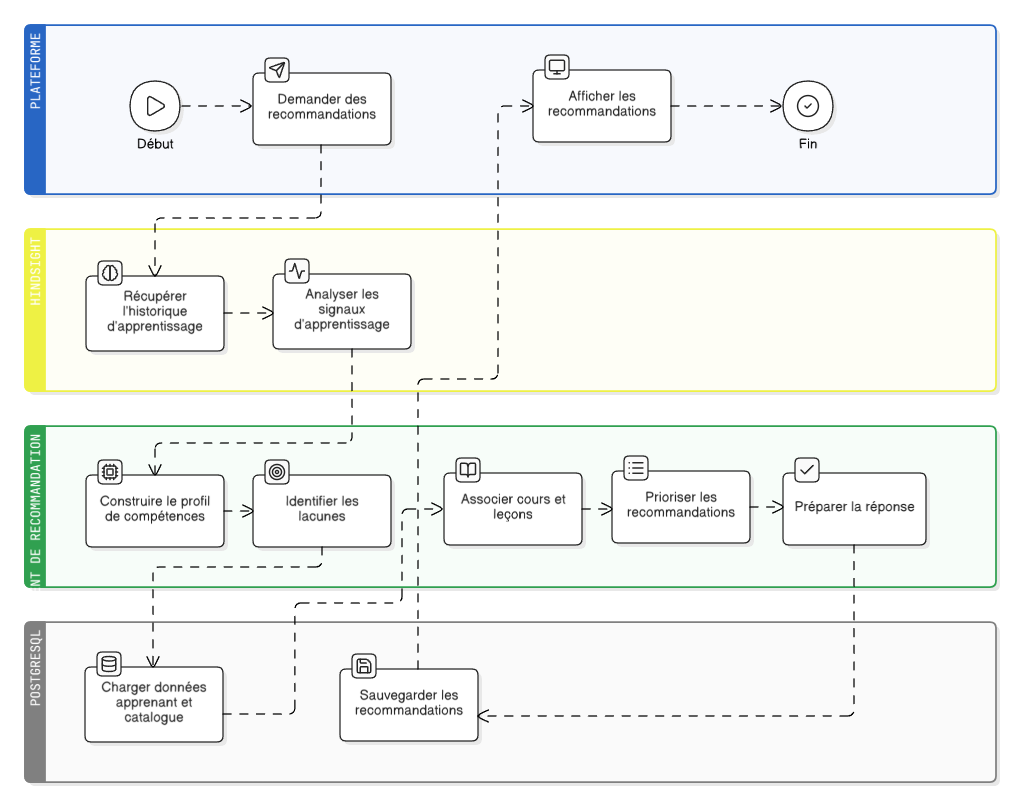
\includegraphics[width=1.05\textwidth,height=0.72\textheight,keepaspectratio]{figures/recommendation_agent_workflow.png}}
    }{%
        \fbox{\parbox{0.85\textwidth}{\centering Diagramme d'activité UML de l'agent de recommandation à insérer ici.}}
    }
    \caption{Diagramme d'activité UML de l'agent de recommandation}
    \label{fig:recommendation_agent_workflow}
\end{figure}

\subsubsection{Agent de défis personnalisés}

Cet agent, appelé \textit{Solo Challenge Agent}, est déclenché automatiquement lors de la connexion de l'utilisateur afin de générer une activité personnalisée visant à renforcer une notion liée à son parcours d'apprentissage. Au démarrage, la plateforme lui transmet les informations d'identification de l'utilisateur, notamment le \textit{tenantId}, le \textit{userId} et le rôle.

L'agent sélectionne ensuite le cours ou le contexte pédagogique le plus pertinent, en privilégiant le dernier cours suivi ou un contenu associé à une difficulté récente non résolue. Il interroge ensuite Hindsight via l'opération \textit{recall} afin de récupérer les informations pertinentes liées à l'apprenant et à son historique d'apprentissage (difficultés, erreurs et signaux pédagogiques).

Sur cette base, l'agent détermine le type de défi à générer. Cette logique est encadrée par des skills spécialisés qui permettent de structurer le comportement de génération sans alourdir le prompt principal. Ces skills sont chargés dynamiquement en fonction du contexte afin d'adapter le défi au profil et à la situation de l'apprenant.

Le résultat généré est une question structurée comprenant un titre, un énoncé, des choix multiples, une réponse correcte et une explication. Avant son affichage, la tentative est enregistrée dans la base de données, et la correction est effectuée lors de la soumission de l'utilisateur. Les résultats sont ensuite réinjectés dans le système de mémoire afin d'améliorer les futures recommandations et générations de défis. Le déroulement détaillé de cet agent est illustré dans la Figure~\ref{fig:solo_challenge_agent_workflow}.

\begin{figure}[H]
    \centering
    \IfFileExists{figures/solo_challenge_agent_workflow.png}{%
        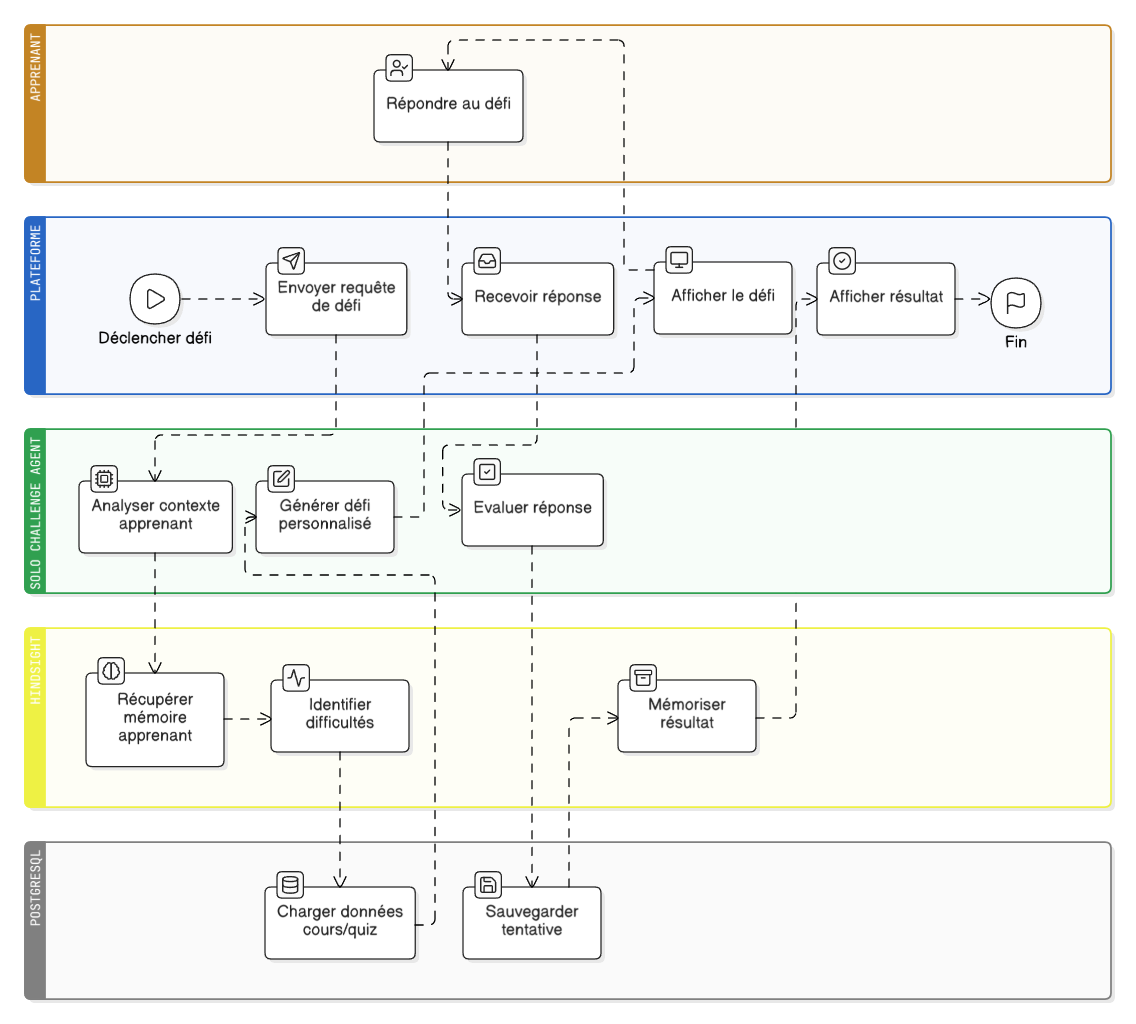
\includegraphics[width=0.95\textwidth,keepaspectratio]{figures/solo_challenge_agent_workflow.png}
    }{%
        \fbox{\parbox{0.85\textwidth}{\centering Diagramme d'activité UML de l'agent de défis personnalisés à insérer ici.}}
    }
    \caption{Diagramme d'activité UML de l'agent de défis personnalisés}
    \label{fig:solo_challenge_agent_workflow}
\end{figure}

En conclusion, cette architecture met en place une couche IA organisée autour de workflows spécialisés et complémentaires. Chaque agent est déclenché dans un contexte précis et produit des résultats exploitables par la plateforme.

Cette séparation permet d'éviter une centralisation de la logique d'intelligence artificielle et garantit un meilleur contrôle du comportement de chaque agent. Elle favorise également une personnalisation progressive du parcours d'apprentissage en s'appuyant sur les interactions réelles de l'utilisateur.

Ainsi, l'IA est intégrée comme une couche fonctionnelle du système, contribuant à l'adaptation et à l'évolution du parcours pédagogique.

\section{Choix technologiques et justification}

Cette section présente les principales technologies retenues pour la réalisation de la plateforme.
L'objectif n'est pas seulement de lister les outils utilisés, mais de justifier leur choix par rapport
aux besoins techniques du projet et aux alternatives possibles.

\subsection{Stack frontend et backend}

La plateforme s'appuie sur une stack technologique adaptée à une architecture microservices intégrant des fonctionnalités d'IA.

Le tableau~\ref{tab:frontend_backend_stack} présente les technologies retenues ainsi que leur justification.

\begin{table}[H]
\centering
\small
\renewcommand{\arraystretch}{1.25}
\caption{Tableau comparatif des technologies frontend et backend retenues}
\label{tab:frontend_backend_stack}
\begin{tabularx}{\textwidth}{|p{2.8cm}|p{4.2cm}|X|}
\hline
\textbf{Technologie} & \textbf{Rôle dans le projet} & \textbf{Justification} \\
\hline
React & Construction des composants de l'interface utilisateur. & React permet de construire des interfaces modulaires à partir de composants réutilisables, ce qui facilite l'organisation des écrans et la maintenance de l'interface. \\
\hline
Next.js & Framework frontend basé sur React pour organiser les pages et les routes. & Next.js apporte une structure applicative au-dessus de React, avec un routage intégré et une meilleure organisation des pages, alors qu'une application React seule nécessite davantage de configuration. \\
\hline
FastAPI & Développement des microservices backend. & FastAPI s'intègre directement avec l'écosystème Python utilisé par les services IA et offre une définition rapide d'API REST typées, alors que NestJS aurait introduit une stack backend Node.js séparée. \\
\hline
Traefik & Routage des requêtes vers les services backend. & Traefik s'intègre facilement avec Docker et permet de centraliser le routage vers les différents services backend à partir de règles déclarées dans l'environnement de déploiement. \\
\hline
\end{tabularx}
\end{table}

\subsection{Bases de données, IA et infrastructure}

Les choix liés au stockage, à la mémoire persistante, aux modèles d'IA et au déploiement ont
été réalisés en fonction des contraintes du projet : cohérence des données, isolation par tenant,
recherche sémantique, simplicité de déploiement et maîtrise des coûts.

Le tableau~\ref{tab:data_ai_infra_stack} synthétise les choix retenus pour les données, l'IA
et l'infrastructure.

\begingroup
\small
\renewcommand{\arraystretch}{1.18}
\begin{longtable}{|p{2.5cm}|p{4cm}|p{9cm}|}
\caption{Tableau comparatif des technologies de données, IA et infrastructure}
\label{tab:data_ai_infra_stack}\\
\hline
\textbf{Technologie} & \textbf{Rôle dans le projet} & \textbf{Justification} \\
\hline
\endfirsthead
\hline
\textbf{Technologie} & \textbf{Rôle dans le projet} & \textbf{Justification} \\
\hline
\endhead
PostgreSQL & Stockage des données relationnelles de la plateforme. & PostgreSQL est adapté aux données fortement liées, comme les utilisateurs, cours, inscriptions et progressions, car il garantit la cohérence relationnelle nécessaire au suivi pédagogique. \\
\hline
pgvector & Stockage et recherche des représentations vectorielles. & pgvector permet d'ajouter la recherche par similarité directement dans PostgreSQL, ce qui simplifie l'infrastructure et évite de maintenir un service de stockage vectoriel indépendant. \\
\hline
MinIO & Stockage objet des fichiers pédagogiques volumineux. & MinIO permet de gérer efficacement les vidéos, images, PDF et supports de cours, tandis que PostgreSQL conserve uniquement les métadonnées et les références vers ces ressources. \\
\hline
Hindsight & Mémoire persistante exploitée par les agents IA. & Hindsight fournit des opérations dédiées à la mémorisation et à la récupération sémantique, ce qui permet d'exploiter une mémoire plus structurée qu'un simple historique de conversation. \\
\hline
Agno OS & Orchestration des agents IA et structuration de leurs workflows. & Agno OS permet de développer et d'orchestrer des agents IA sous forme de services spécialisés. Cette approche favorise la modularité, la maintenabilité et l'intégration des fonctionnalités IA dans la plateforme. \\
\hline
OpenRouter / LLM & Accès au modèle de langage principal utilisé par les fonctionnalités IA. & OpenRouter permet d'utiliser un modèle performant et accessible hors réseau interne, tout en conservant le modèle local de l'entreprise comme solution de secours lorsque le contexte le permet. \\
\hline
RabbitMQ & Gestion des échanges asynchrones entre certains services. & RabbitMQ permet de traiter des événements métier sans bloquer directement le parcours utilisateur, ce qui convient aux notifications et aux traitements déclenchés en arrière-plan. \\
\hline
Redis & Stockage temporaire de contextes préparés pour certains agents IA. & Redis est adapté aux données intermédiaires et temporaires, tandis que PostgreSQL reste réservé aux données métier persistantes nécessitant une cohérence relationnelle. \\
\hline
Piper & Génération audio locale pour la synthèse vocale des contenus. & Piper permet de produire des voix de synthèse dans l'environnement de déploiement, ce qui limite la dépendance à un service externe pour la génération audio. \\
\hline
Docker / Docker Compose & Conteneurisation et orchestration locale des services de la plateforme. & Docker isole les services dans des conteneurs reproductibles, tandis que Docker Compose facilite leur lancement coordonné dans un même environnement. \\
\hline
\end{longtable}
\endgroup

\section{Conclusion}

Ce chapitre a présenté la conception de la plateforme ainsi que les principaux choix architecturaux et technologiques retenus. Il a permis de décrire l'organisation générale du système, son architecture microservices, son approche multi-tenant, son modèle de données et l'intégration des agents d'intelligence artificielle.

Cette conception constitue le cadre de référence pour la mise en œuvre de la solution. Le chapitre suivant est consacré à la réalisation de la plateforme, à la présentation des différents modules développés ainsi qu'à son déploiement et son hébergement.
\endinput
